\section{The Git structure}
The git is divided mainly in three components. The working directory,
the index and the repository. The connection between this components
can be seen in figure \ref{fig:git_structure}. 

\begin{figure}[h!]
   \centering
   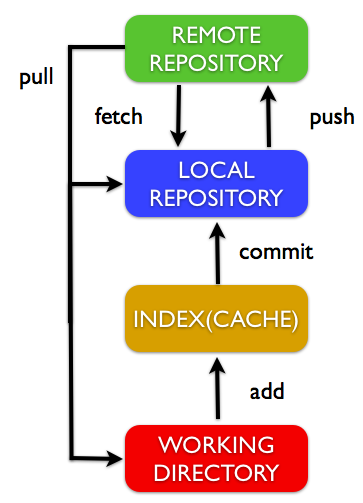
\includegraphics[width=0.5\textwidth]{images/data_flow_simplified.png}
   \caption{Git Structure}\label{fig:git_structure}
\end{figure}

The working directory is a subset of
a file system that contains the files of the project that you are
currently working on. When retrieving an older snapshot of the project, the
working directory is updated to reflect the project that state. The index is a
component between the repository and the working directory. It
contains the files that will be on the next commit
(on the next snapshot). Finally the repository is like a database. It contains 
all the information about your system, all the snapshots taken till
the moment. In figure \ref{fig:git_structure} there are a local
repository and a remote repository. In reality there are no difference
between them, they have the same structure. Both of them are local
repository, and at the same time remote repository. Each one sees the 
other as remote repository.\\

For a matter of time and complexity, in this project we turned our attention 
mainly to the index and repository. We are not modeling what is going
on in the working directory. We just model that there are files in the
working directory, anything else.
